% First-pass design workflow (Chapter 7, sec:foundation).
% Compile: pdflatex -output-directory=.. design_workflow.tex
% All action boxes are imperatives; inputs are noun phrases. Wide column
% pitch so the input-arrow labels fit their gaps with clearance.
\documentclass[border=6pt]{standalone}
\usepackage[T1]{fontenc}
\usepackage{mathpazo}
\usepackage{tikz}
\usetikzlibrary{arrows.meta, positioning, calc, shapes.geometric}
\begin{document}
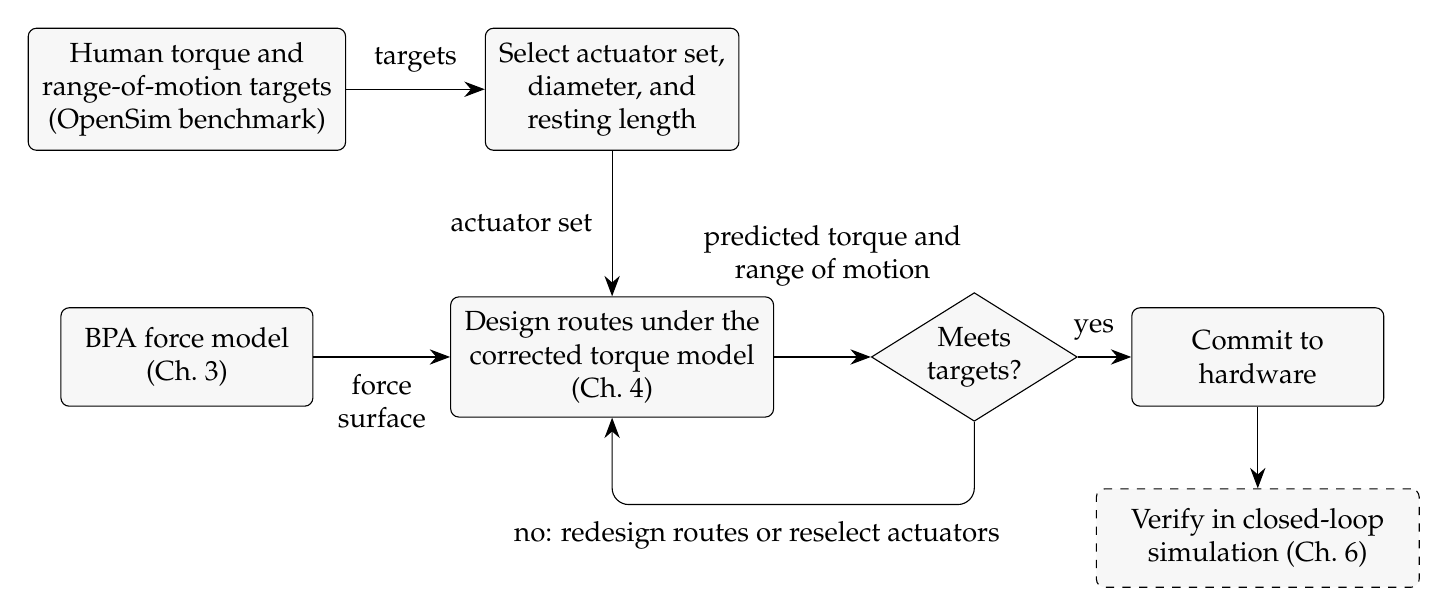
\begin{tikzpicture}[
  font=\normalsize,
  box/.style={draw, rounded corners=3pt, align=center, inner sep=5pt,
              minimum width=3.2cm, minimum height=1.25cm, fill=black!3},
  verify/.style={box, dashed, minimum width=4.1cm},
  dec/.style={draw, diamond, aspect=1.6, align=center, inner sep=1pt,
              fill=black!3, minimum width=2.1cm, minimum height=1.3cm},
  arrow/.style={-{Stealth[length=2.6mm]}, thin, rounded corners=6pt},
  lab/.style={align=center, inner sep=3pt},
]

% Row 1: inputs to selection
\node[box] (targets) at (-0.6,0)  {Human torque and\\range-of-motion targets\\(OpenSim benchmark)};
\node[box] (select)  at (4.8,0)   {Select actuator set,\\diameter, and\\resting length};
% Row 2: force model to routing
\node[box] (bpamodel) at (-0.6,-3.4) {BPA force model\\(Ch.~3)};
\node[box] (route)    at (4.8,-3.4){Design routes under the\\corrected torque model\\(Ch.~4)};
% Decision row
\node[dec]  (meets)  at (9.4,-3.4)  {Meets\\targets?};
\node[box]  (commit) at (13.0,-3.4) {Commit to\\hardware};
\node[verify] (verify) at (13.0,-5.7) {Verify in closed-loop\\simulation (Ch.~6)};

\draw[arrow] (targets.east) -- node[lab, above=3pt] {targets} (select.west);
\draw[arrow] (bpamodel.east) -- node[lab, below=3pt] {force\\surface} (route.west);
\draw[arrow] (select) -- node[lab, left=4pt] {actuator set} (route);
\draw[arrow] (route.east) -- (meets.west);
\node[lab, anchor=south] at (7.60,-2.62) {predicted torque and\\range of motion};
\draw[arrow] (meets.east) -- node[lab, above=3pt, pos=0.30] {yes} (commit.west);
\draw[arrow] (meets.south) -- ++(0,-1.05) -| node[lab, pos=0.30, below=3pt]
  {no: redesign routes or reselect actuators} (route.south);
\draw[arrow] (commit) -- (verify);

\end{tikzpicture}
\end{document}
